% Created by tikzDevice version 0.6.2-92-0ad2792 on 2013-03-03 12:19:44
% !TEX encoding = UTF-8 Unicode
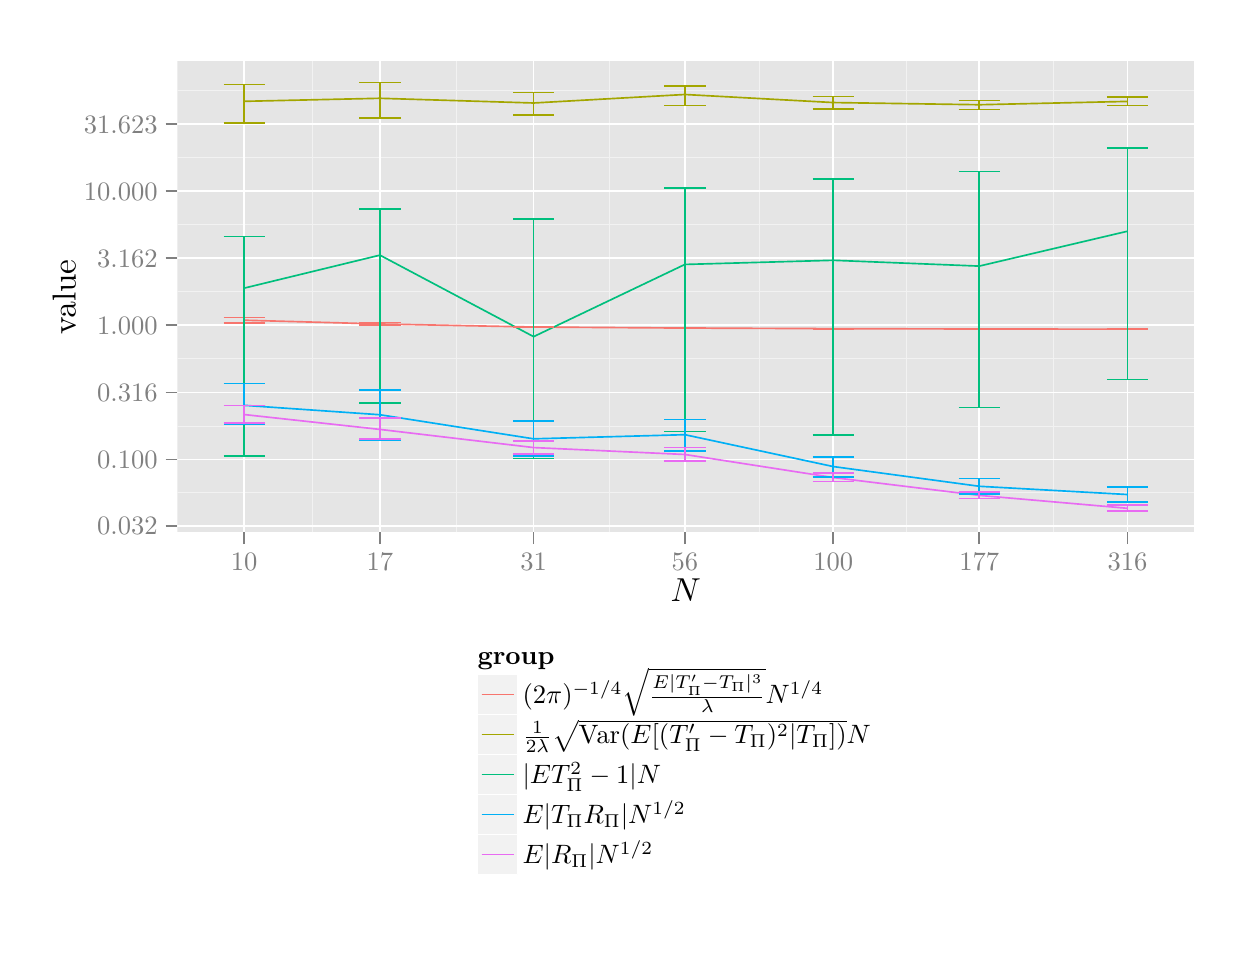
\begin{tikzpicture}[x=1pt,y=1pt]
\definecolor[named]{fillColor}{rgb}{1.00,1.00,1.00}
\path[use as bounding box,fill=fillColor,fill opacity=0.00] (0,0) rectangle (433.62,325.21);
\begin{scope}
\path[clip] (  0.00,  0.00) rectangle (433.62,325.21);
\definecolor[named]{drawColor}{rgb}{1.00,1.00,1.00}
\definecolor[named]{fillColor}{rgb}{1.00,1.00,1.00}

\path[draw=drawColor,line width= 0.6pt,line join=round,line cap=round,fill=fillColor] (  0.00,  0.00) rectangle (433.62,325.21);
\end{scope}
\begin{scope}
\path[clip] ( 54.08,142.81) rectangle (421.57,313.17);
\definecolor[named]{fillColor}{rgb}{0.90,0.90,0.90}

\path[fill=fillColor] ( 54.08,142.81) rectangle (421.57,313.17);
\definecolor[named]{drawColor}{rgb}{0.95,0.95,0.95}

\path[draw=drawColor,line width= 0.3pt,line join=round] ( 54.08,157.19) --
	(421.57,157.19);

\path[draw=drawColor,line width= 0.3pt,line join=round] ( 54.08,181.30) --
	(421.57,181.30);

\path[draw=drawColor,line width= 0.3pt,line join=round] ( 54.08,205.55) --
	(421.57,205.55);

\path[draw=drawColor,line width= 0.3pt,line join=round] ( 54.08,229.79) --
	(421.57,229.79);

\path[draw=drawColor,line width= 0.3pt,line join=round] ( 54.08,254.04) --
	(421.57,254.04);

\path[draw=drawColor,line width= 0.3pt,line join=round] ( 54.08,278.28) --
	(421.57,278.28);

\path[draw=drawColor,line width= 0.3pt,line join=round] ( 54.08,302.39) --
	(421.57,302.39);

\path[draw=drawColor,line width= 0.3pt,line join=round] (102.76,142.81) --
	(102.76,313.17);

\path[draw=drawColor,line width= 0.3pt,line join=round] (155.05,142.81) --
	(155.05,313.17);

\path[draw=drawColor,line width= 0.3pt,line join=round] (210.15,142.81) --
	(210.15,313.17);

\path[draw=drawColor,line width= 0.3pt,line join=round] (264.27,142.81) --
	(264.27,313.17);

\path[draw=drawColor,line width= 0.3pt,line join=round] (317.46,142.81) --
	(317.46,313.17);

\path[draw=drawColor,line width= 0.3pt,line join=round] (370.63,142.81) --
	(370.63,313.17);
\definecolor[named]{drawColor}{rgb}{1.00,1.00,1.00}

\path[draw=drawColor,line width= 0.6pt,line join=round] ( 54.08,145.20) --
	(421.57,145.20);

\path[draw=drawColor,line width= 0.6pt,line join=round] ( 54.08,169.19) --
	(421.57,169.19);

\path[draw=drawColor,line width= 0.6pt,line join=round] ( 54.08,193.42) --
	(421.57,193.42);

\path[draw=drawColor,line width= 0.6pt,line join=round] ( 54.08,217.67) --
	(421.57,217.67);

\path[draw=drawColor,line width= 0.6pt,line join=round] ( 54.08,241.91) --
	(421.57,241.91);

\path[draw=drawColor,line width= 0.6pt,line join=round] ( 54.08,266.16) --
	(421.57,266.16);

\path[draw=drawColor,line width= 0.6pt,line join=round] ( 54.08,290.40) --
	(421.57,290.40);

\path[draw=drawColor,line width= 0.6pt,line join=round] ( 78.24,142.81) --
	( 78.24,313.17);

\path[draw=drawColor,line width= 0.6pt,line join=round] (127.28,142.81) --
	(127.28,313.17);

\path[draw=drawColor,line width= 0.6pt,line join=round] (182.82,142.81) --
	(182.82,313.17);

\path[draw=drawColor,line width= 0.6pt,line join=round] (237.48,142.81) --
	(237.48,313.17);

\path[draw=drawColor,line width= 0.6pt,line join=round] (291.07,142.81) --
	(291.07,313.17);

\path[draw=drawColor,line width= 0.6pt,line join=round] (343.85,142.81) --
	(343.85,313.17);

\path[draw=drawColor,line width= 0.6pt,line join=round] (397.42,142.81) --
	(397.42,313.17);
\definecolor[named]{drawColor}{rgb}{0.97,0.46,0.43}

\path[draw=drawColor,line width= 0.6pt,line join=round] ( 78.24,219.50) --
	(127.28,218.14) --
	(182.82,217.04) --
	(237.48,216.66) --
	(291.07,216.45) --
	(343.85,216.32) --
	(397.42,216.27);
\definecolor[named]{drawColor}{rgb}{0.64,0.65,0.00}

\path[draw=drawColor,line width= 0.6pt,line join=round] ( 78.24,298.59) --
	(127.28,299.69) --
	(182.82,297.99) --
	(237.48,301.06) --
	(291.07,298.15) --
	(343.85,297.36) --
	(397.42,298.56);
\definecolor[named]{drawColor}{rgb}{0.00,0.75,0.49}

\path[draw=drawColor,line width= 0.6pt,line join=round] ( 78.24,231.09) --
	(127.28,243.01) --
	(182.82,213.56) --
	(237.48,239.65) --
	(291.07,241.15) --
	(343.85,239.05) --
	(397.42,251.65);
\definecolor[named]{drawColor}{rgb}{0.00,0.69,0.96}

\path[draw=drawColor,line width= 0.6pt,line join=round] ( 78.24,188.74) --
	(127.28,185.34) --
	(182.82,176.64) --
	(237.48,178.13) --
	(291.07,166.62) --
	(343.85,159.49) --
	(397.42,156.51);
\definecolor[named]{drawColor}{rgb}{0.91,0.42,0.95}

\path[draw=drawColor,line width= 0.6pt,line join=round] ( 78.24,185.41) --
	(127.28,180.04) --
	(182.82,173.48) --
	(237.48,170.98) --
	(291.07,162.65) --
	(343.85,156.20) --
	(397.42,151.53);
\definecolor[named]{drawColor}{rgb}{0.97,0.46,0.43}

\path[draw=drawColor,line width= 0.6pt,line join=round] ( 70.79,220.53) --
	( 85.69,220.53);

\path[draw=drawColor,line width= 0.6pt,line join=round] ( 78.24,220.53) --
	( 78.24,218.57);

\path[draw=drawColor,line width= 0.6pt,line join=round] ( 70.79,218.57) --
	( 85.69,218.57);

\path[draw=drawColor,line width= 0.6pt,line join=round] (119.83,218.63) --
	(134.73,218.63);

\path[draw=drawColor,line width= 0.6pt,line join=round] (127.28,218.63) --
	(127.28,217.66);

\path[draw=drawColor,line width= 0.6pt,line join=round] (119.83,217.66) --
	(134.73,217.66);

\path[draw=drawColor,line width= 0.6pt,line join=round] (175.37,217.24) --
	(190.26,217.24);

\path[draw=drawColor,line width= 0.6pt,line join=round] (182.82,217.24) --
	(182.82,216.88);

\path[draw=drawColor,line width= 0.6pt,line join=round] (175.37,216.88) --
	(190.26,216.88);

\path[draw=drawColor,line width= 0.6pt,line join=round] (230.03,216.75) --
	(244.93,216.75);

\path[draw=drawColor,line width= 0.6pt,line join=round] (237.48,216.75) --
	(237.48,216.58);

\path[draw=drawColor,line width= 0.6pt,line join=round] (230.03,216.58) --
	(244.93,216.58);

\path[draw=drawColor,line width= 0.6pt,line join=round] (283.62,216.48) --
	(298.52,216.48);

\path[draw=drawColor,line width= 0.6pt,line join=round] (291.07,216.48) --
	(291.07,216.42);

\path[draw=drawColor,line width= 0.6pt,line join=round] (283.62,216.42) --
	(298.52,216.42);

\path[draw=drawColor,line width= 0.6pt,line join=round] (336.40,216.34) --
	(351.30,216.34);

\path[draw=drawColor,line width= 0.6pt,line join=round] (343.85,216.34) --
	(343.85,216.31);

\path[draw=drawColor,line width= 0.6pt,line join=round] (336.40,216.31) --
	(351.30,216.31);

\path[draw=drawColor,line width= 0.6pt,line join=round] (389.97,216.27) --
	(404.87,216.27);

\path[draw=drawColor,line width= 0.6pt,line join=round] (397.42,216.27) --
	(397.42,216.26);

\path[draw=drawColor,line width= 0.6pt,line join=round] (389.97,216.26) --
	(404.87,216.26);
\definecolor[named]{drawColor}{rgb}{0.64,0.65,0.00}

\path[draw=drawColor,line width= 0.6pt,line join=round] ( 70.79,304.71) --
	( 85.69,304.71);

\path[draw=drawColor,line width= 0.6pt,line join=round] ( 78.24,304.71) --
	( 78.24,290.67);

\path[draw=drawColor,line width= 0.6pt,line join=round] ( 70.79,290.67) --
	( 85.69,290.67);

\path[draw=drawColor,line width= 0.6pt,line join=round] (119.83,305.43) --
	(134.73,305.43);

\path[draw=drawColor,line width= 0.6pt,line join=round] (127.28,305.43) --
	(127.28,292.47);

\path[draw=drawColor,line width= 0.6pt,line join=round] (119.83,292.47) --
	(134.73,292.47);

\path[draw=drawColor,line width= 0.6pt,line join=round] (175.37,301.82) --
	(190.26,301.82);

\path[draw=drawColor,line width= 0.6pt,line join=round] (182.82,301.82) --
	(182.82,293.57);

\path[draw=drawColor,line width= 0.6pt,line join=round] (175.37,293.57) --
	(190.26,293.57);

\path[draw=drawColor,line width= 0.6pt,line join=round] (230.03,304.17) --
	(244.93,304.17);

\path[draw=drawColor,line width= 0.6pt,line join=round] (237.48,304.17) --
	(237.48,297.04);

\path[draw=drawColor,line width= 0.6pt,line join=round] (230.03,297.04) --
	(244.93,297.04);

\path[draw=drawColor,line width= 0.6pt,line join=round] (283.62,300.33) --
	(298.52,300.33);

\path[draw=drawColor,line width= 0.6pt,line join=round] (291.07,300.33) --
	(291.07,295.85);

\path[draw=drawColor,line width= 0.6pt,line join=round] (283.62,295.85) --
	(298.52,295.85);

\path[draw=drawColor,line width= 0.6pt,line join=round] (336.40,298.90) --
	(351.30,298.90);

\path[draw=drawColor,line width= 0.6pt,line join=round] (343.85,298.90) --
	(343.85,295.66);

\path[draw=drawColor,line width= 0.6pt,line join=round] (336.40,295.66) --
	(351.30,295.66);

\path[draw=drawColor,line width= 0.6pt,line join=round] (389.97,300.09) --
	(404.87,300.09);

\path[draw=drawColor,line width= 0.6pt,line join=round] (397.42,300.09) --
	(397.42,297.05);

\path[draw=drawColor,line width= 0.6pt,line join=round] (389.97,297.05) --
	(404.87,297.05);
\definecolor[named]{drawColor}{rgb}{0.00,0.75,0.49}

\path[draw=drawColor,line width= 0.6pt,line join=round] ( 70.79,249.72) --
	( 85.69,249.72);

\path[draw=drawColor,line width= 0.6pt,line join=round] ( 78.24,249.72) --
	( 78.24,170.32);

\path[draw=drawColor,line width= 0.6pt,line join=round] ( 70.79,170.32) --
	( 85.69,170.32);

\path[draw=drawColor,line width= 0.6pt,line join=round] (119.83,259.70) --
	(134.73,259.70);

\path[draw=drawColor,line width= 0.6pt,line join=round] (127.28,259.70) --
	(127.28,189.55);

\path[draw=drawColor,line width= 0.6pt,line join=round] (119.83,189.55) --
	(134.73,189.55);

\path[draw=drawColor,line width= 0.6pt,line join=round] (175.37,256.11) --
	(190.26,256.11);

\path[draw=drawColor,line width= 0.6pt,line join=round] (182.82,256.11) --
	(182.82,169.48);

\path[draw=drawColor,line width= 0.6pt,line join=round] (175.37,169.48) --
	(190.26,169.48);

\path[draw=drawColor,line width= 0.6pt,line join=round] (230.03,267.33) --
	(244.93,267.33);

\path[draw=drawColor,line width= 0.6pt,line join=round] (237.48,267.33) --
	(237.48,179.30);

\path[draw=drawColor,line width= 0.6pt,line join=round] (230.03,179.30) --
	(244.93,179.30);

\path[draw=drawColor,line width= 0.6pt,line join=round] (283.62,270.49) --
	(298.52,270.49);

\path[draw=drawColor,line width= 0.6pt,line join=round] (291.07,270.49) --
	(291.07,178.00);

\path[draw=drawColor,line width= 0.6pt,line join=round] (283.62,178.00) --
	(298.52,178.00);

\path[draw=drawColor,line width= 0.6pt,line join=round] (336.40,273.22) --
	(351.30,273.22);

\path[draw=drawColor,line width= 0.6pt,line join=round] (343.85,273.22) --
	(343.85,187.93);

\path[draw=drawColor,line width= 0.6pt,line join=round] (336.40,187.93) --
	(351.30,187.93);

\path[draw=drawColor,line width= 0.6pt,line join=round] (389.97,281.82) --
	(404.87,281.82);

\path[draw=drawColor,line width= 0.6pt,line join=round] (397.42,281.82) --
	(397.42,198.04);

\path[draw=drawColor,line width= 0.6pt,line join=round] (389.97,198.04) --
	(404.87,198.04);
\definecolor[named]{drawColor}{rgb}{0.00,0.69,0.96}

\path[draw=drawColor,line width= 0.6pt,line join=round] ( 70.79,196.65) --
	( 85.69,196.65);

\path[draw=drawColor,line width= 0.6pt,line join=round] ( 78.24,196.65) --
	( 78.24,181.85);

\path[draw=drawColor,line width= 0.6pt,line join=round] ( 70.79,181.85) --
	( 85.69,181.85);

\path[draw=drawColor,line width= 0.6pt,line join=round] (119.83,194.34) --
	(134.73,194.34);

\path[draw=drawColor,line width= 0.6pt,line join=round] (127.28,194.34) --
	(127.28,176.33);

\path[draw=drawColor,line width= 0.6pt,line join=round] (119.83,176.33) --
	(134.73,176.33);

\path[draw=drawColor,line width= 0.6pt,line join=round] (175.37,183.03) --
	(190.26,183.03);

\path[draw=drawColor,line width= 0.6pt,line join=round] (182.82,183.03) --
	(182.82,170.53);

\path[draw=drawColor,line width= 0.6pt,line join=round] (175.37,170.53) --
	(190.26,170.53);

\path[draw=drawColor,line width= 0.6pt,line join=round] (230.03,183.62) --
	(244.93,183.62);

\path[draw=drawColor,line width= 0.6pt,line join=round] (237.48,183.62) --
	(237.48,172.24);

\path[draw=drawColor,line width= 0.6pt,line join=round] (230.03,172.24) --
	(244.93,172.24);

\path[draw=drawColor,line width= 0.6pt,line join=round] (283.62,170.15) --
	(298.52,170.15);

\path[draw=drawColor,line width= 0.6pt,line join=round] (291.07,170.15) --
	(291.07,162.78);

\path[draw=drawColor,line width= 0.6pt,line join=round] (283.62,162.78) --
	(298.52,162.78);

\path[draw=drawColor,line width= 0.6pt,line join=round] (336.40,162.32) --
	(351.30,162.32);

\path[draw=drawColor,line width= 0.6pt,line join=round] (343.85,162.32) --
	(343.85,156.81);

\path[draw=drawColor,line width= 0.6pt,line join=round] (336.40,156.81) --
	(351.30,156.81);

\path[draw=drawColor,line width= 0.6pt,line join=round] (389.97,159.27) --
	(404.87,159.27);

\path[draw=drawColor,line width= 0.6pt,line join=round] (397.42,159.27) --
	(397.42,153.87);

\path[draw=drawColor,line width= 0.6pt,line join=round] (389.97,153.87) --
	(404.87,153.87);
\definecolor[named]{drawColor}{rgb}{0.91,0.42,0.95}

\path[draw=drawColor,line width= 0.6pt,line join=round] ( 70.79,188.69) --
	( 85.69,188.69);

\path[draw=drawColor,line width= 0.6pt,line join=round] ( 78.24,188.69) --
	( 78.24,182.34);

\path[draw=drawColor,line width= 0.6pt,line join=round] ( 70.79,182.34) --
	( 85.69,182.34);

\path[draw=drawColor,line width= 0.6pt,line join=round] (119.83,184.19) --
	(134.73,184.19);

\path[draw=drawColor,line width= 0.6pt,line join=round] (127.28,184.19) --
	(127.28,176.63);

\path[draw=drawColor,line width= 0.6pt,line join=round] (119.83,176.63) --
	(134.73,176.63);

\path[draw=drawColor,line width= 0.6pt,line join=round] (175.37,175.97) --
	(190.26,175.97);

\path[draw=drawColor,line width= 0.6pt,line join=round] (182.82,175.97) --
	(182.82,171.19);

\path[draw=drawColor,line width= 0.6pt,line join=round] (175.37,171.19) --
	(190.26,171.19);

\path[draw=drawColor,line width= 0.6pt,line join=round] (230.03,173.52) --
	(244.93,173.52);

\path[draw=drawColor,line width= 0.6pt,line join=round] (237.48,173.52) --
	(237.48,168.61);

\path[draw=drawColor,line width= 0.6pt,line join=round] (230.03,168.61) --
	(244.93,168.61);

\path[draw=drawColor,line width= 0.6pt,line join=round] (283.62,164.24) --
	(298.52,164.24);

\path[draw=drawColor,line width= 0.6pt,line join=round] (291.07,164.24) --
	(291.07,161.19);

\path[draw=drawColor,line width= 0.6pt,line join=round] (283.62,161.19) --
	(298.52,161.19);

\path[draw=drawColor,line width= 0.6pt,line join=round] (336.40,157.34) --
	(351.30,157.34);

\path[draw=drawColor,line width= 0.6pt,line join=round] (343.85,157.34) --
	(343.85,155.09);

\path[draw=drawColor,line width= 0.6pt,line join=round] (336.40,155.09) --
	(351.30,155.09);

\path[draw=drawColor,line width= 0.6pt,line join=round] (389.97,152.63) --
	(404.87,152.63);

\path[draw=drawColor,line width= 0.6pt,line join=round] (397.42,152.63) --
	(397.42,150.56);

\path[draw=drawColor,line width= 0.6pt,line join=round] (389.97,150.56) --
	(404.87,150.56);
\end{scope}
\begin{scope}
\path[clip] (  0.00,  0.00) rectangle (433.62,325.21);
\definecolor[named]{drawColor}{rgb}{0.50,0.50,0.50}

\node[text=drawColor,anchor=base east,inner sep=0pt, outer sep=0pt, scale=  0.96] at ( 46.97,141.89) {0.032};

\node[text=drawColor,anchor=base east,inner sep=0pt, outer sep=0pt, scale=  0.96] at ( 46.97,165.88) {0.100};

\node[text=drawColor,anchor=base east,inner sep=0pt, outer sep=0pt, scale=  0.96] at ( 46.97,190.11) {0.316};

\node[text=drawColor,anchor=base east,inner sep=0pt, outer sep=0pt, scale=  0.96] at ( 46.97,214.37) {1.000};

\node[text=drawColor,anchor=base east,inner sep=0pt, outer sep=0pt, scale=  0.96] at ( 46.97,238.61) {3.162};

\node[text=drawColor,anchor=base east,inner sep=0pt, outer sep=0pt, scale=  0.96] at ( 46.97,262.85) {10.000};

\node[text=drawColor,anchor=base east,inner sep=0pt, outer sep=0pt, scale=  0.96] at ( 46.97,287.09) {31.623};
\end{scope}
\begin{scope}
\path[clip] (  0.00,  0.00) rectangle (433.62,325.21);
\definecolor[named]{drawColor}{rgb}{0.50,0.50,0.50}

\path[draw=drawColor,line width= 0.6pt,line join=round] ( 49.82,145.20) --
	( 54.08,145.20);

\path[draw=drawColor,line width= 0.6pt,line join=round] ( 49.82,169.19) --
	( 54.08,169.19);

\path[draw=drawColor,line width= 0.6pt,line join=round] ( 49.82,193.42) --
	( 54.08,193.42);

\path[draw=drawColor,line width= 0.6pt,line join=round] ( 49.82,217.67) --
	( 54.08,217.67);

\path[draw=drawColor,line width= 0.6pt,line join=round] ( 49.82,241.91) --
	( 54.08,241.91);

\path[draw=drawColor,line width= 0.6pt,line join=round] ( 49.82,266.16) --
	( 54.08,266.16);

\path[draw=drawColor,line width= 0.6pt,line join=round] ( 49.82,290.40) --
	( 54.08,290.40);
\end{scope}
\begin{scope}
\path[clip] (  0.00,  0.00) rectangle (433.62,325.21);
\definecolor[named]{drawColor}{rgb}{0.50,0.50,0.50}

\path[draw=drawColor,line width= 0.6pt,line join=round] ( 78.24,138.55) --
	( 78.24,142.81);

\path[draw=drawColor,line width= 0.6pt,line join=round] (127.28,138.55) --
	(127.28,142.81);

\path[draw=drawColor,line width= 0.6pt,line join=round] (182.82,138.55) --
	(182.82,142.81);

\path[draw=drawColor,line width= 0.6pt,line join=round] (237.48,138.55) --
	(237.48,142.81);

\path[draw=drawColor,line width= 0.6pt,line join=round] (291.07,138.55) --
	(291.07,142.81);

\path[draw=drawColor,line width= 0.6pt,line join=round] (343.85,138.55) --
	(343.85,142.81);

\path[draw=drawColor,line width= 0.6pt,line join=round] (397.42,138.55) --
	(397.42,142.81);
\end{scope}
\begin{scope}
\path[clip] (  0.00,  0.00) rectangle (433.62,325.21);
\definecolor[named]{drawColor}{rgb}{0.50,0.50,0.50}

\node[text=drawColor,anchor=base,inner sep=0pt, outer sep=0pt, scale=  0.96] at ( 78.24,129.09) {10};

\node[text=drawColor,anchor=base,inner sep=0pt, outer sep=0pt, scale=  0.96] at (127.28,129.09) {17};

\node[text=drawColor,anchor=base,inner sep=0pt, outer sep=0pt, scale=  0.96] at (182.82,129.09) {31};

\node[text=drawColor,anchor=base,inner sep=0pt, outer sep=0pt, scale=  0.96] at (237.48,129.09) {56};

\node[text=drawColor,anchor=base,inner sep=0pt, outer sep=0pt, scale=  0.96] at (291.07,129.09) {100};

\node[text=drawColor,anchor=base,inner sep=0pt, outer sep=0pt, scale=  0.96] at (343.85,129.09) {177};

\node[text=drawColor,anchor=base,inner sep=0pt, outer sep=0pt, scale=  0.96] at (397.42,129.09) {316};
\end{scope}
\begin{scope}
\path[clip] (  0.00,  0.00) rectangle (433.62,325.21);
\definecolor[named]{drawColor}{rgb}{0.00,0.00,0.00}

\node[text=drawColor,anchor=base,inner sep=0pt, outer sep=0pt, scale=  1.20] at (237.83,117.81) {$N$};
\end{scope}
\begin{scope}
\path[clip] (  0.00,  0.00) rectangle (433.62,325.21);
\definecolor[named]{drawColor}{rgb}{0.00,0.00,0.00}

\node[text=drawColor,rotate= 90.00,anchor=base,inner sep=0pt, outer sep=0pt, scale=  1.20] at ( 17.30,227.99) {value};
\end{scope}
\begin{scope}
\path[clip] (  0.00,  0.00) rectangle (433.62,325.21);
\definecolor[named]{fillColor}{rgb}{1.00,1.00,1.00}

\path[fill=fillColor] (158.31, 14.89) rectangle (317.35,105.93);
\end{scope}
\begin{scope}
\path[clip] (  0.00,  0.00) rectangle (433.62,325.21);
\definecolor[named]{drawColor}{rgb}{0.00,0.00,0.00}

\node[text=drawColor,anchor=base west,inner sep=0pt, outer sep=0pt, scale=  0.96] at (162.58, 95.04) {\bfseries group};
\end{scope}
\begin{scope}
\path[clip] (  0.00,  0.00) rectangle (433.62,325.21);
\definecolor[named]{drawColor}{rgb}{1.00,1.00,1.00}
\definecolor[named]{fillColor}{rgb}{0.95,0.95,0.95}

\path[draw=drawColor,line width= 0.6pt,line join=round,line cap=round,fill=fillColor] (162.58, 76.97) rectangle (177.03, 91.43);
\end{scope}
\begin{scope}
\path[clip] (  0.00,  0.00) rectangle (433.62,325.21);
\definecolor[named]{drawColor}{rgb}{0.97,0.46,0.43}

\path[draw=drawColor,line width= 0.6pt,line join=round] (164.02, 84.20) -- (175.58, 84.20);
\end{scope}
\begin{scope}
\path[clip] (  0.00,  0.00) rectangle (433.62,325.21);
\definecolor[named]{drawColor}{rgb}{0.97,0.46,0.43}

\path[draw=drawColor,line width= 0.6pt,line join=round] (164.02, 84.20) -- (175.58, 84.20);
\end{scope}
\begin{scope}
\path[clip] (  0.00,  0.00) rectangle (433.62,325.21);
\definecolor[named]{drawColor}{rgb}{1.00,1.00,1.00}
\definecolor[named]{fillColor}{rgb}{0.95,0.95,0.95}

\path[draw=drawColor,line width= 0.6pt,line join=round,line cap=round,fill=fillColor] (162.58, 62.52) rectangle (177.03, 76.97);
\end{scope}
\begin{scope}
\path[clip] (  0.00,  0.00) rectangle (433.62,325.21);
\definecolor[named]{drawColor}{rgb}{0.64,0.65,0.00}

\path[draw=drawColor,line width= 0.6pt,line join=round] (164.02, 69.75) -- (175.58, 69.75);
\end{scope}
\begin{scope}
\path[clip] (  0.00,  0.00) rectangle (433.62,325.21);
\definecolor[named]{drawColor}{rgb}{0.64,0.65,0.00}

\path[draw=drawColor,line width= 0.6pt,line join=round] (164.02, 69.75) -- (175.58, 69.75);
\end{scope}
\begin{scope}
\path[clip] (  0.00,  0.00) rectangle (433.62,325.21);
\definecolor[named]{drawColor}{rgb}{1.00,1.00,1.00}
\definecolor[named]{fillColor}{rgb}{0.95,0.95,0.95}

\path[draw=drawColor,line width= 0.6pt,line join=round,line cap=round,fill=fillColor] (162.58, 48.07) rectangle (177.03, 62.52);
\end{scope}
\begin{scope}
\path[clip] (  0.00,  0.00) rectangle (433.62,325.21);
\definecolor[named]{drawColor}{rgb}{0.00,0.75,0.49}

\path[draw=drawColor,line width= 0.6pt,line join=round] (164.02, 55.29) -- (175.58, 55.29);
\end{scope}
\begin{scope}
\path[clip] (  0.00,  0.00) rectangle (433.62,325.21);
\definecolor[named]{drawColor}{rgb}{0.00,0.75,0.49}

\path[draw=drawColor,line width= 0.6pt,line join=round] (164.02, 55.29) -- (175.58, 55.29);
\end{scope}
\begin{scope}
\path[clip] (  0.00,  0.00) rectangle (433.62,325.21);
\definecolor[named]{drawColor}{rgb}{1.00,1.00,1.00}
\definecolor[named]{fillColor}{rgb}{0.95,0.95,0.95}

\path[draw=drawColor,line width= 0.6pt,line join=round,line cap=round,fill=fillColor] (162.58, 33.61) rectangle (177.03, 48.07);
\end{scope}
\begin{scope}
\path[clip] (  0.00,  0.00) rectangle (433.62,325.21);
\definecolor[named]{drawColor}{rgb}{0.00,0.69,0.96}

\path[draw=drawColor,line width= 0.6pt,line join=round] (164.02, 40.84) -- (175.58, 40.84);
\end{scope}
\begin{scope}
\path[clip] (  0.00,  0.00) rectangle (433.62,325.21);
\definecolor[named]{drawColor}{rgb}{0.00,0.69,0.96}

\path[draw=drawColor,line width= 0.6pt,line join=round] (164.02, 40.84) -- (175.58, 40.84);
\end{scope}
\begin{scope}
\path[clip] (  0.00,  0.00) rectangle (433.62,325.21);
\definecolor[named]{drawColor}{rgb}{1.00,1.00,1.00}
\definecolor[named]{fillColor}{rgb}{0.95,0.95,0.95}

\path[draw=drawColor,line width= 0.6pt,line join=round,line cap=round,fill=fillColor] (162.58, 19.16) rectangle (177.03, 33.61);
\end{scope}
\begin{scope}
\path[clip] (  0.00,  0.00) rectangle (433.62,325.21);
\definecolor[named]{drawColor}{rgb}{0.91,0.42,0.95}

\path[draw=drawColor,line width= 0.6pt,line join=round] (164.02, 26.39) -- (175.58, 26.39);
\end{scope}
\begin{scope}
\path[clip] (  0.00,  0.00) rectangle (433.62,325.21);
\definecolor[named]{drawColor}{rgb}{0.91,0.42,0.95}

\path[draw=drawColor,line width= 0.6pt,line join=round] (164.02, 26.39) -- (175.58, 26.39);
\end{scope}
\begin{scope}
\path[clip] (  0.00,  0.00) rectangle (433.62,325.21);
\definecolor[named]{drawColor}{rgb}{0.00,0.00,0.00}

\node[text=drawColor,anchor=base west,inner sep=0pt, outer sep=0pt, scale=  0.96] at (178.84, 80.90) {$(2\pi)^{-1/4}\sqrt{\frac{\mathbb{E}|T'_{\Pi}-T_{\Pi}|^3}{\lambda}}N^{1/4}\quad $};
\end{scope}
\begin{scope}
\path[clip] (  0.00,  0.00) rectangle (433.62,325.21);
\definecolor[named]{drawColor}{rgb}{0.00,0.00,0.00}

\node[text=drawColor,anchor=base west,inner sep=0pt, outer sep=0pt, scale=  0.96] at (178.84, 66.44) {$\frac{1}{2\lambda}\sqrt{\mathrm{Var}(\mathbb{E}[(T'_{\Pi}-T_{\Pi})^2|T_{\Pi}])}N\quad $};
\end{scope}
\begin{scope}
\path[clip] (  0.00,  0.00) rectangle (433.62,325.21);
\definecolor[named]{drawColor}{rgb}{0.00,0.00,0.00}

\node[text=drawColor,anchor=base west,inner sep=0pt, outer sep=0pt, scale=  0.96] at (178.84, 51.99) {$|\mathbb{E}T_{\Pi}^2-1|N\quad $};
\end{scope}
\begin{scope}
\path[clip] (  0.00,  0.00) rectangle (433.62,325.21);
\definecolor[named]{drawColor}{rgb}{0.00,0.00,0.00}

\node[text=drawColor,anchor=base west,inner sep=0pt, outer sep=0pt, scale=  0.96] at (178.84, 37.53) {$\mathbb{E}|T_{\Pi}R_{\Pi}|N^{1/2}\quad $};
\end{scope}
\begin{scope}
\path[clip] (  0.00,  0.00) rectangle (433.62,325.21);
\definecolor[named]{drawColor}{rgb}{0.00,0.00,0.00}

\node[text=drawColor,anchor=base west,inner sep=0pt, outer sep=0pt, scale=  0.96] at (178.84, 23.08) {$\mathbb{E}|R_{\Pi}|N^{1/2}\quad $};
\end{scope}
\end{tikzpicture}
